\documentclass[12pt]{article}

\usepackage{amsmath}
\usepackage{amssymb}
\usepackage{amsthm}
\usepackage{mathtools}
\usepackage{mathrsfs}
\usepackage{hyperref}
\usepackage{braket}
\usepackage{bm}
\usepackage{graphicx}
\usepackage[
    left = 1in,
    right = 1in,
    top = 1in,
    bottom = 1in
]{geometry}
\usepackage{titling}
\usepackage{parskip}
\usepackage{hyperref}
\usepackage{fancyhdr}
\usepackage{caption}

\graphicspath{{Attachments/}}

\pagestyle{fancy}
\fancyhf{}
\rhead{\small AC Multivariable Calculus}
\lhead{\small Final Project}
\cfoot{\thepage}
\renewcommand{\headrulewidth}{0.4pt}
\fancyfoot{}
\renewcommand{\footrulewidth}{0.4pt}
\rfoot{\small \thepage}
\lfoot{\small Adams, Meng, Harpavat, and Charoenrattanaruk}
\setlength{\headheight}{13.59999pt}

\title{\textbf{Multivariable Calculus Final Project}}
\author{Diego, Michael, Keshav, and Parrie}
\date{}

\begin{document}

\maketitle
\thispagestyle{fancy}

\tableofcontents

\clearpage

\section{Construction}

\subsection{Introduction \& Design}

For this project, our group chose a cone with radius $30"$ and height $36"$ (or
$2.5'$ and $3'$, respectively). The equation that we used was 
\begin{equation*}
    \frac{x^{2}}{225} + \frac{y^{2}}{225} = \frac{z^{2}}{900},
\end{equation*}
where $x \in [-15, 15]$, $y \in [-15, 15]$, and $z \in [0, 30]$. Our cone was
domain-restricted to only positive $z$ values, as it would be physically very
difficult to construct a cone that extended into the ground.

\subsection{Construction Process}

We decided to construct an cone with a peak radius of $15"$ and a peak height of
$30"$, with the peak radius at the base. To construct the cone, we used wooden
sticks to prop up the circles that represented certain radii, and we used metal
wire to create those circles. We originally planned to construct a cone with
peak radius $30"$ and a peak height of $36"$, but Diego pointed out that such a
cone would exceed the dimensions of the project area.

\begin{figure}[h!]
    \centering
    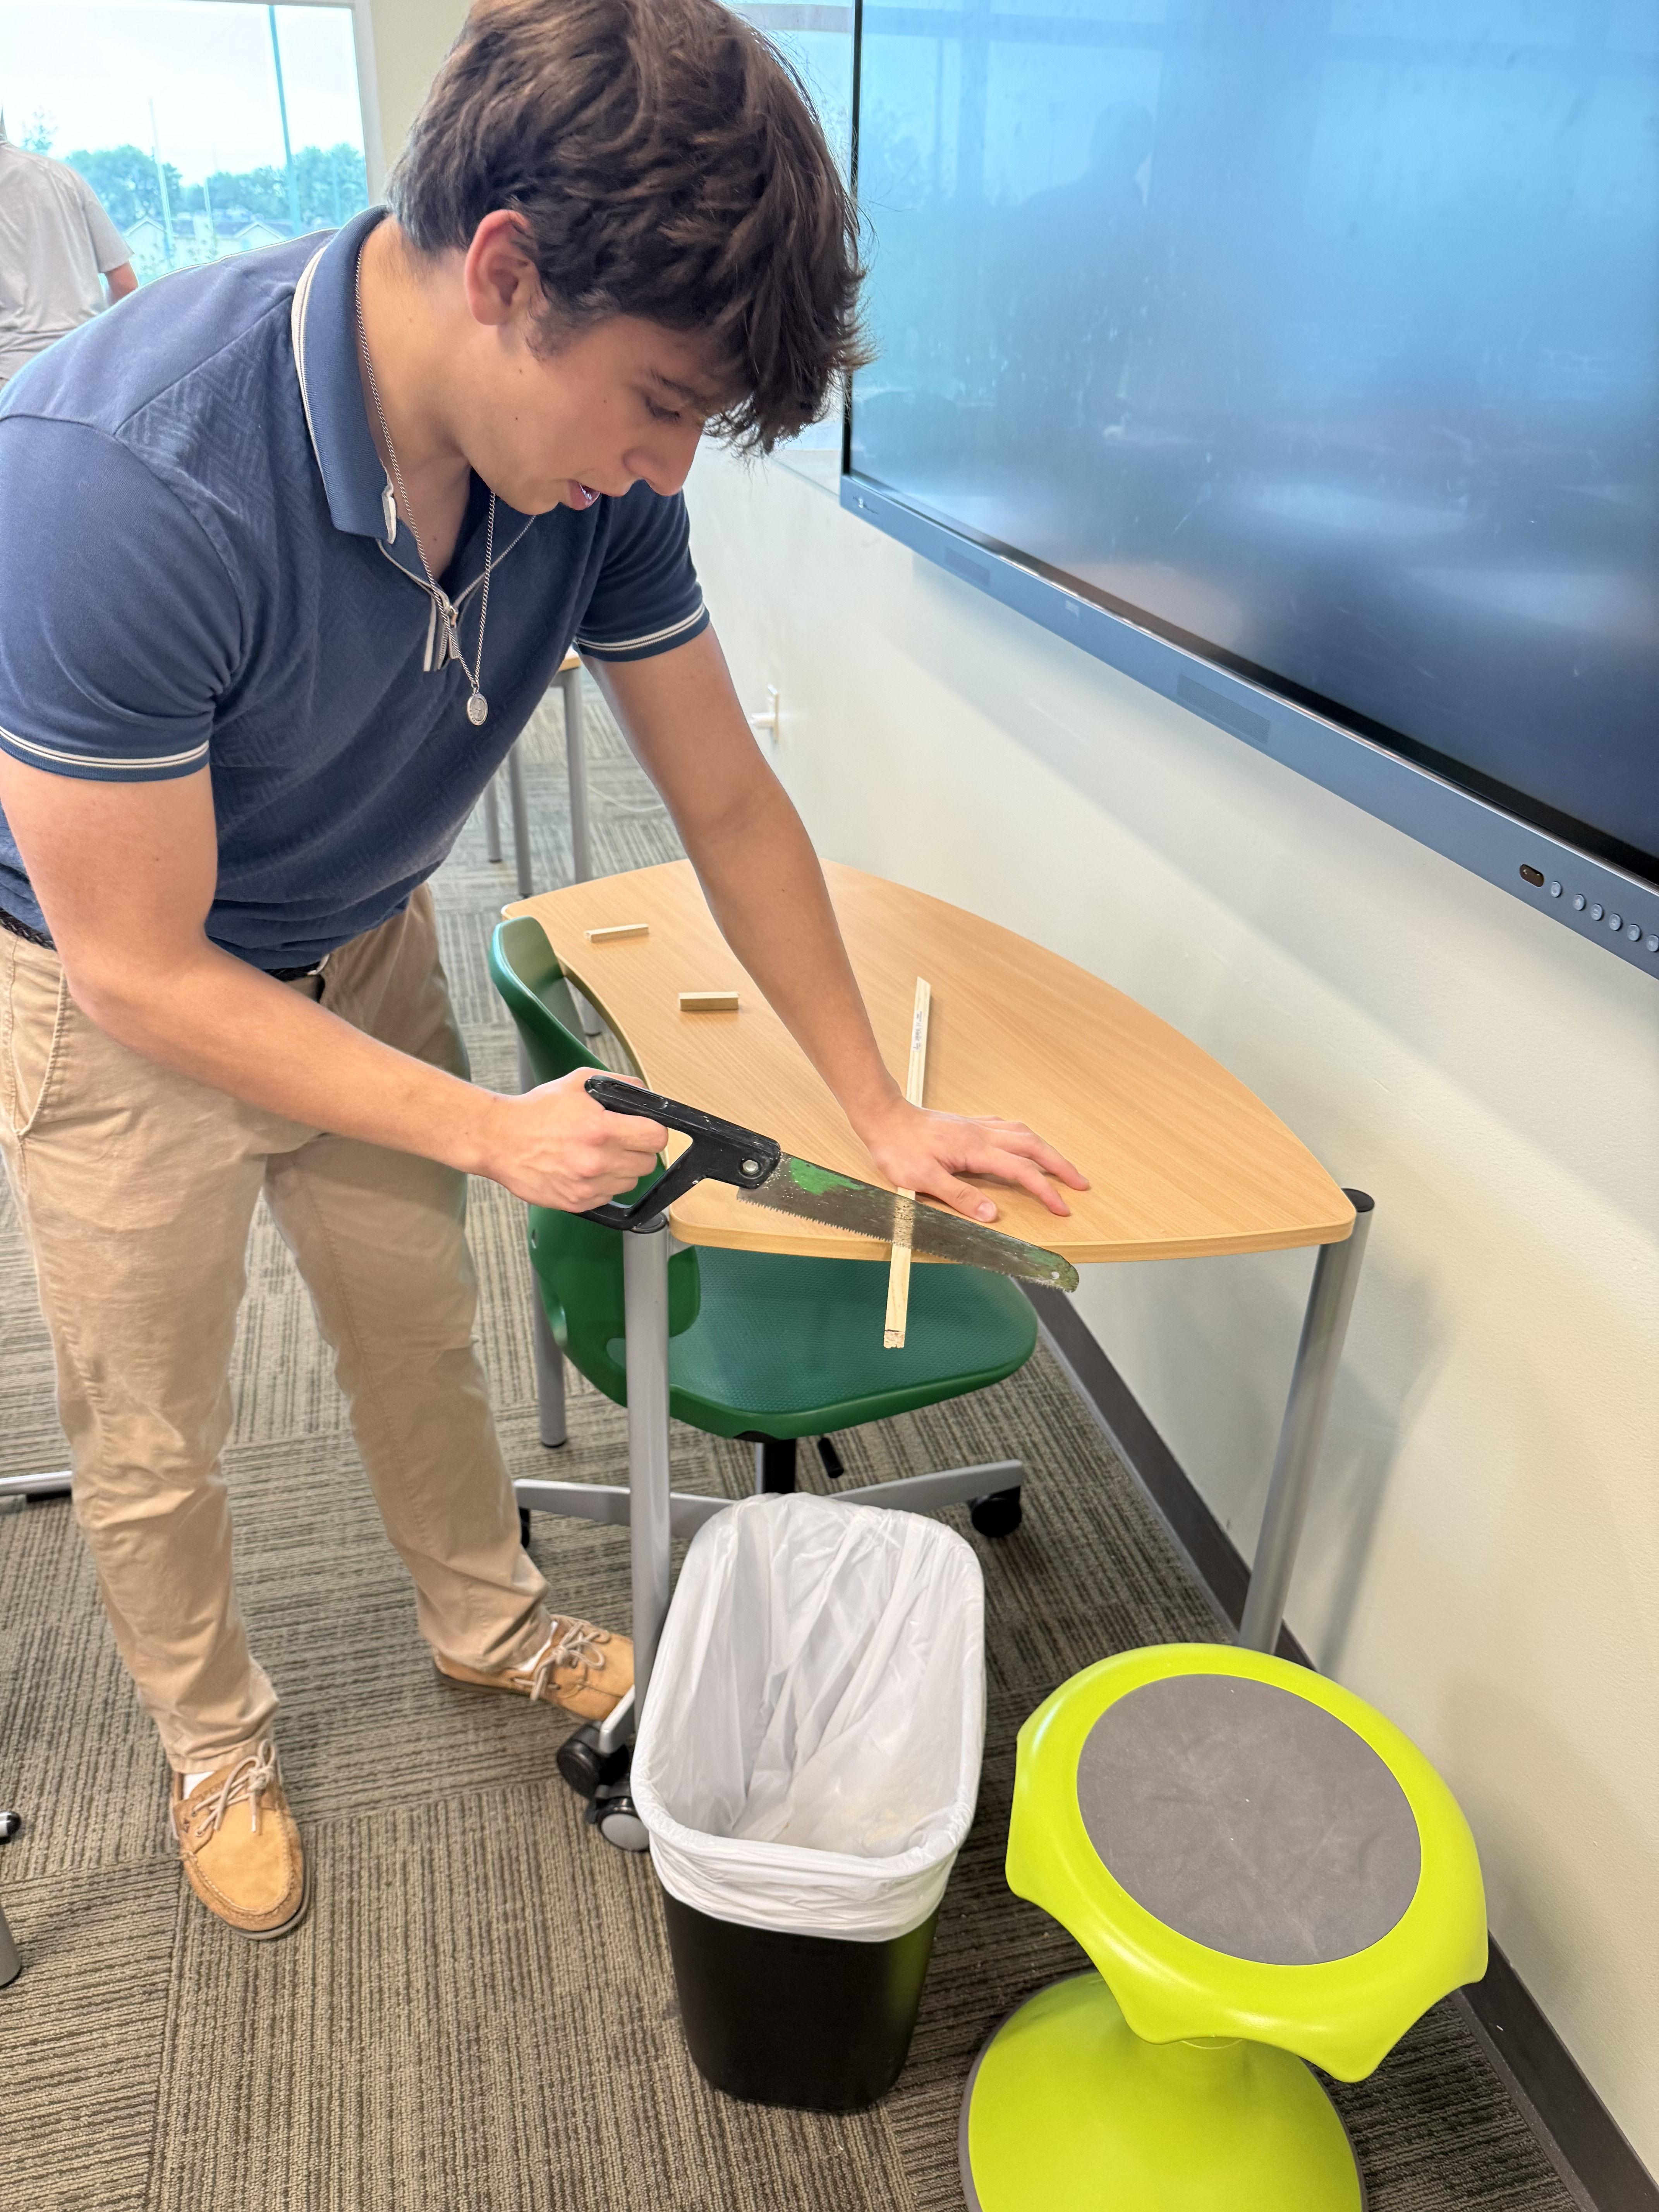
\includegraphics[width=0.5\textwidth]{diego-sawing-wood.jpg}
    \caption*{Diego sawing the wooden support sticks.}
    \label{fig:diego-sawing-wood}
\end{figure}

The construction process consisted of measuring out the radii for the wire
circles and placing the wooden sticks on the outer sides of the cone to then
place those wires on. The construction process required sawing the wooden
sticks, which were at first too long, to the proper lengths to fit on the edges,
or hypotenuses, approximately $33.5"$.

\begin{figure}[h!]
    \centering
    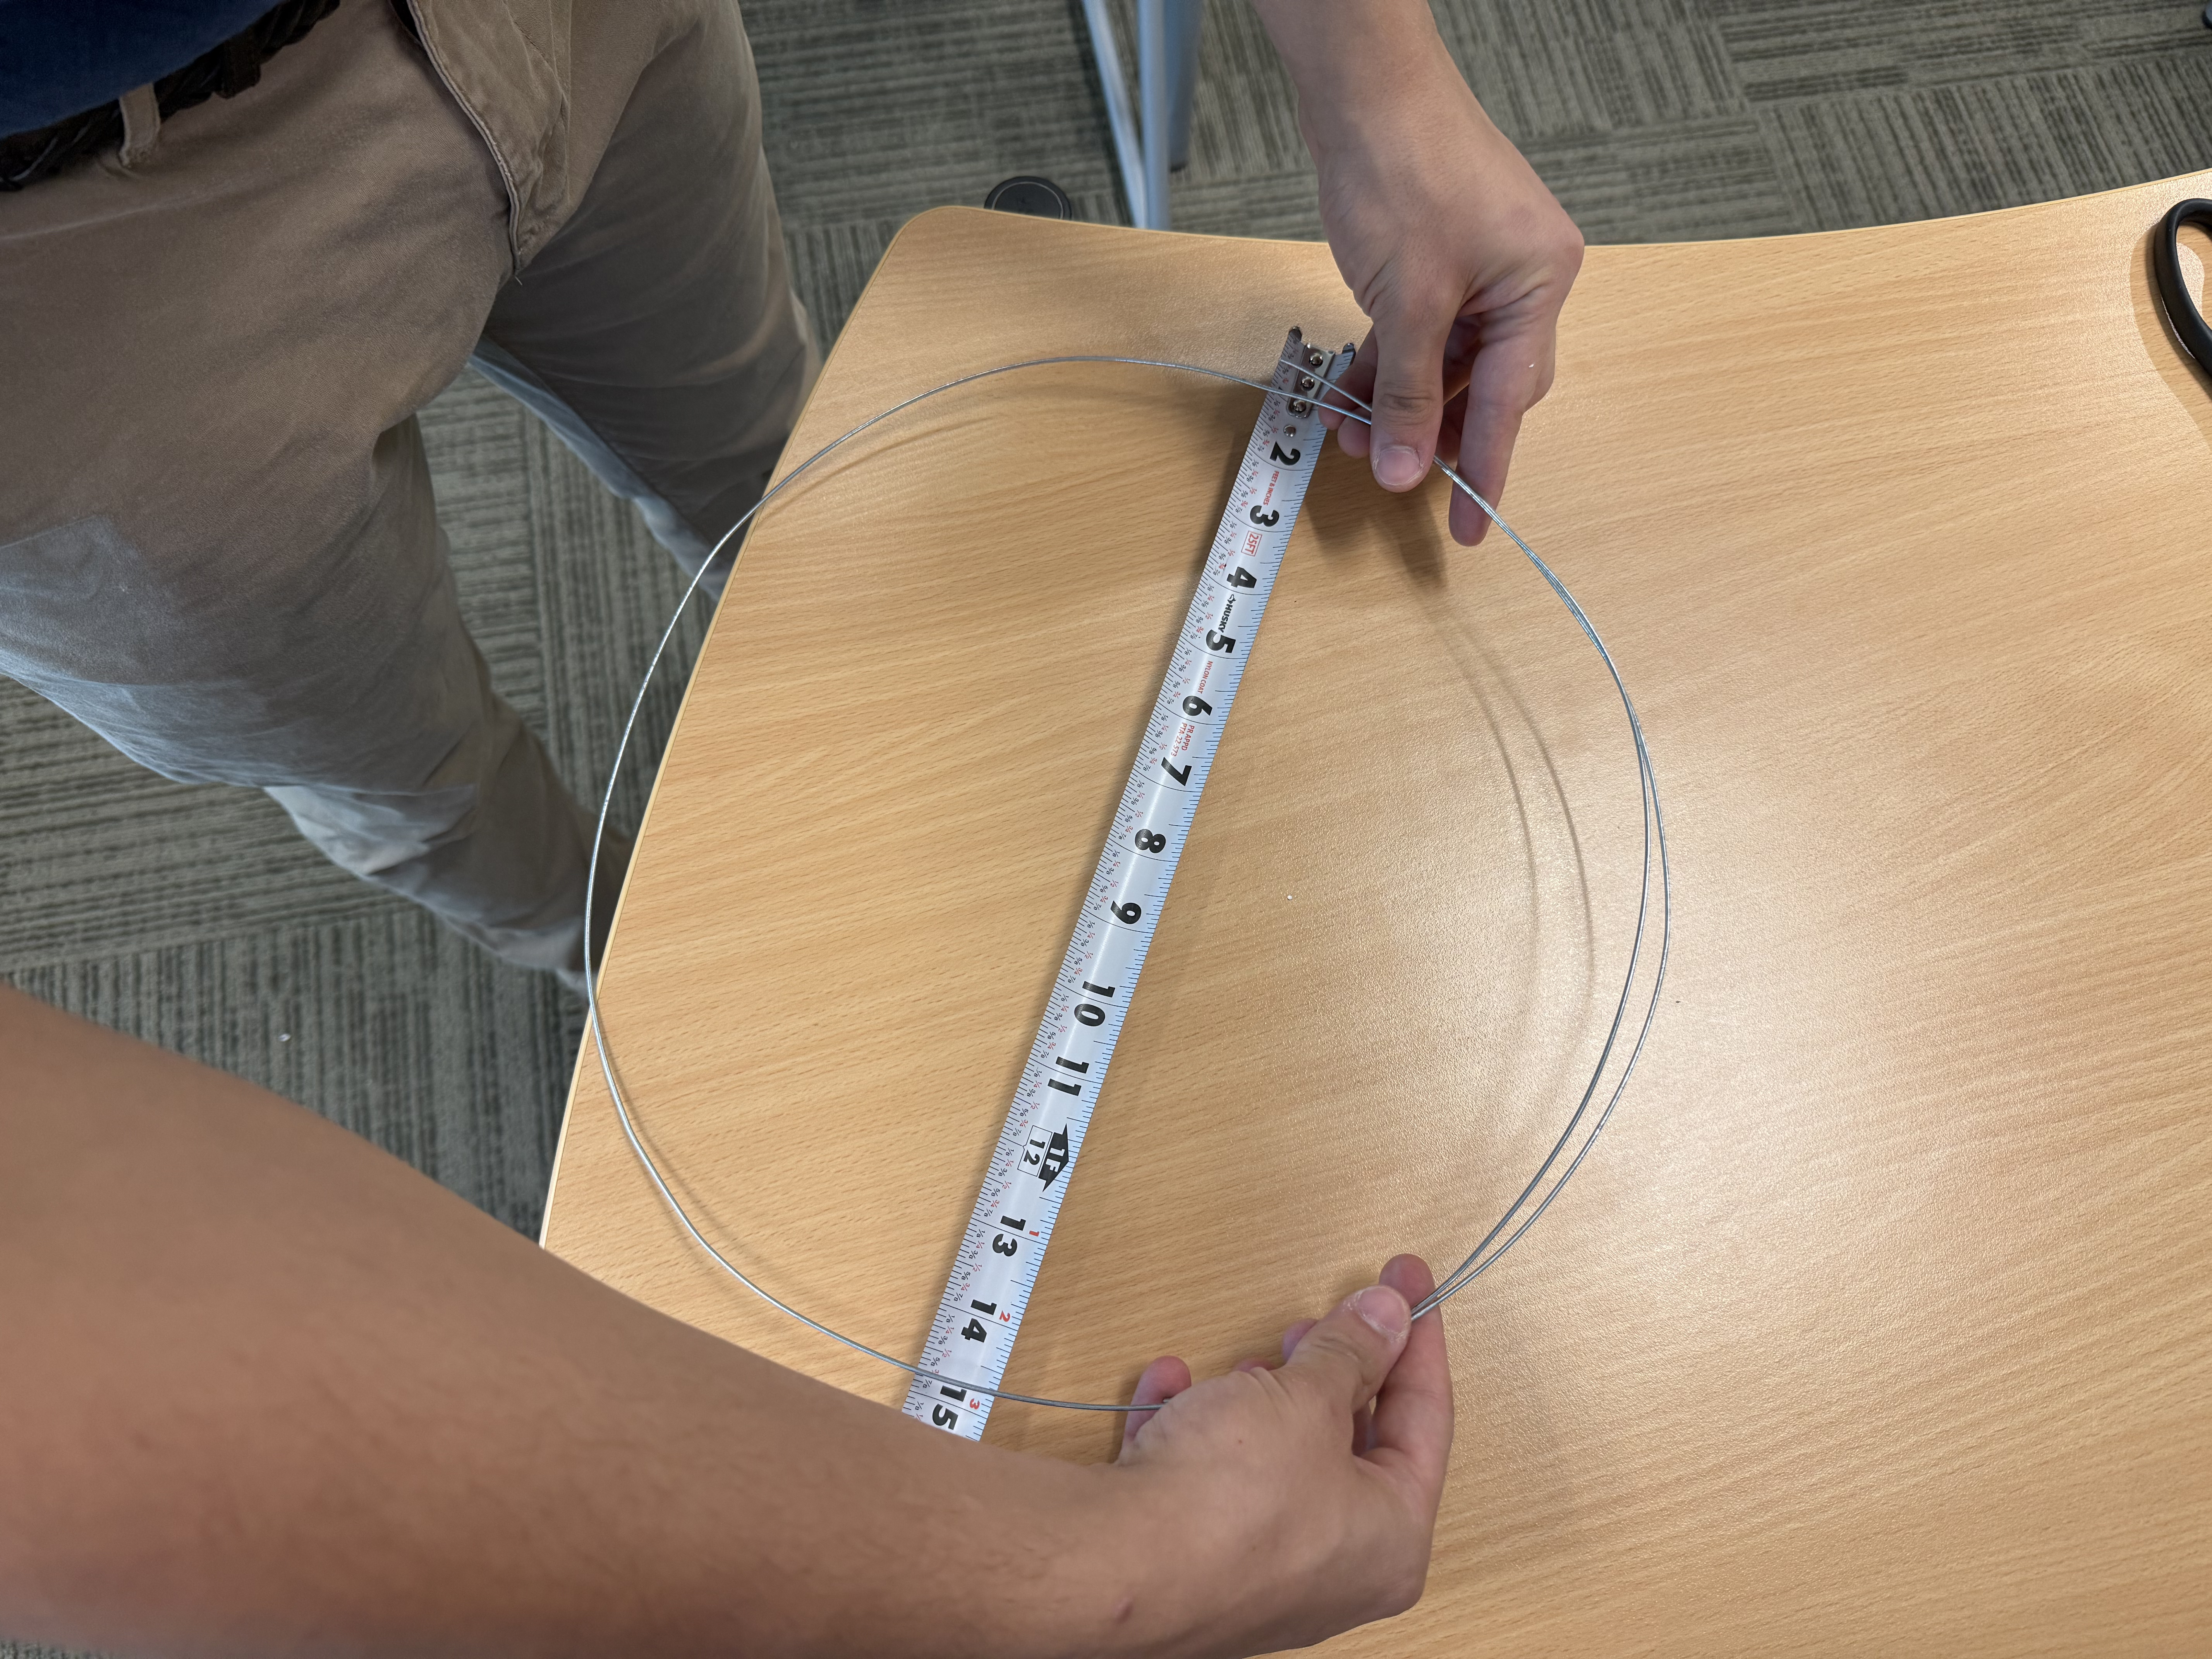
\includegraphics[width=0.5\textwidth]{circle-measurement}
    \caption*{Diego measuring a circle for the cone.}
    \label{fig:circle-measurement}
\end{figure}

Our construction eventually yielded a finished cone, with five wire circles
around the middle and hypotenuse poles. We used wood glue and some, generously,
tape to hold everything down. We also asked another group for their extra foam
pieces for the platform and borrowed some wooden poles and steel wire.
Basically, we survived on communism.

\begin{figure}[h!]
    \centering
    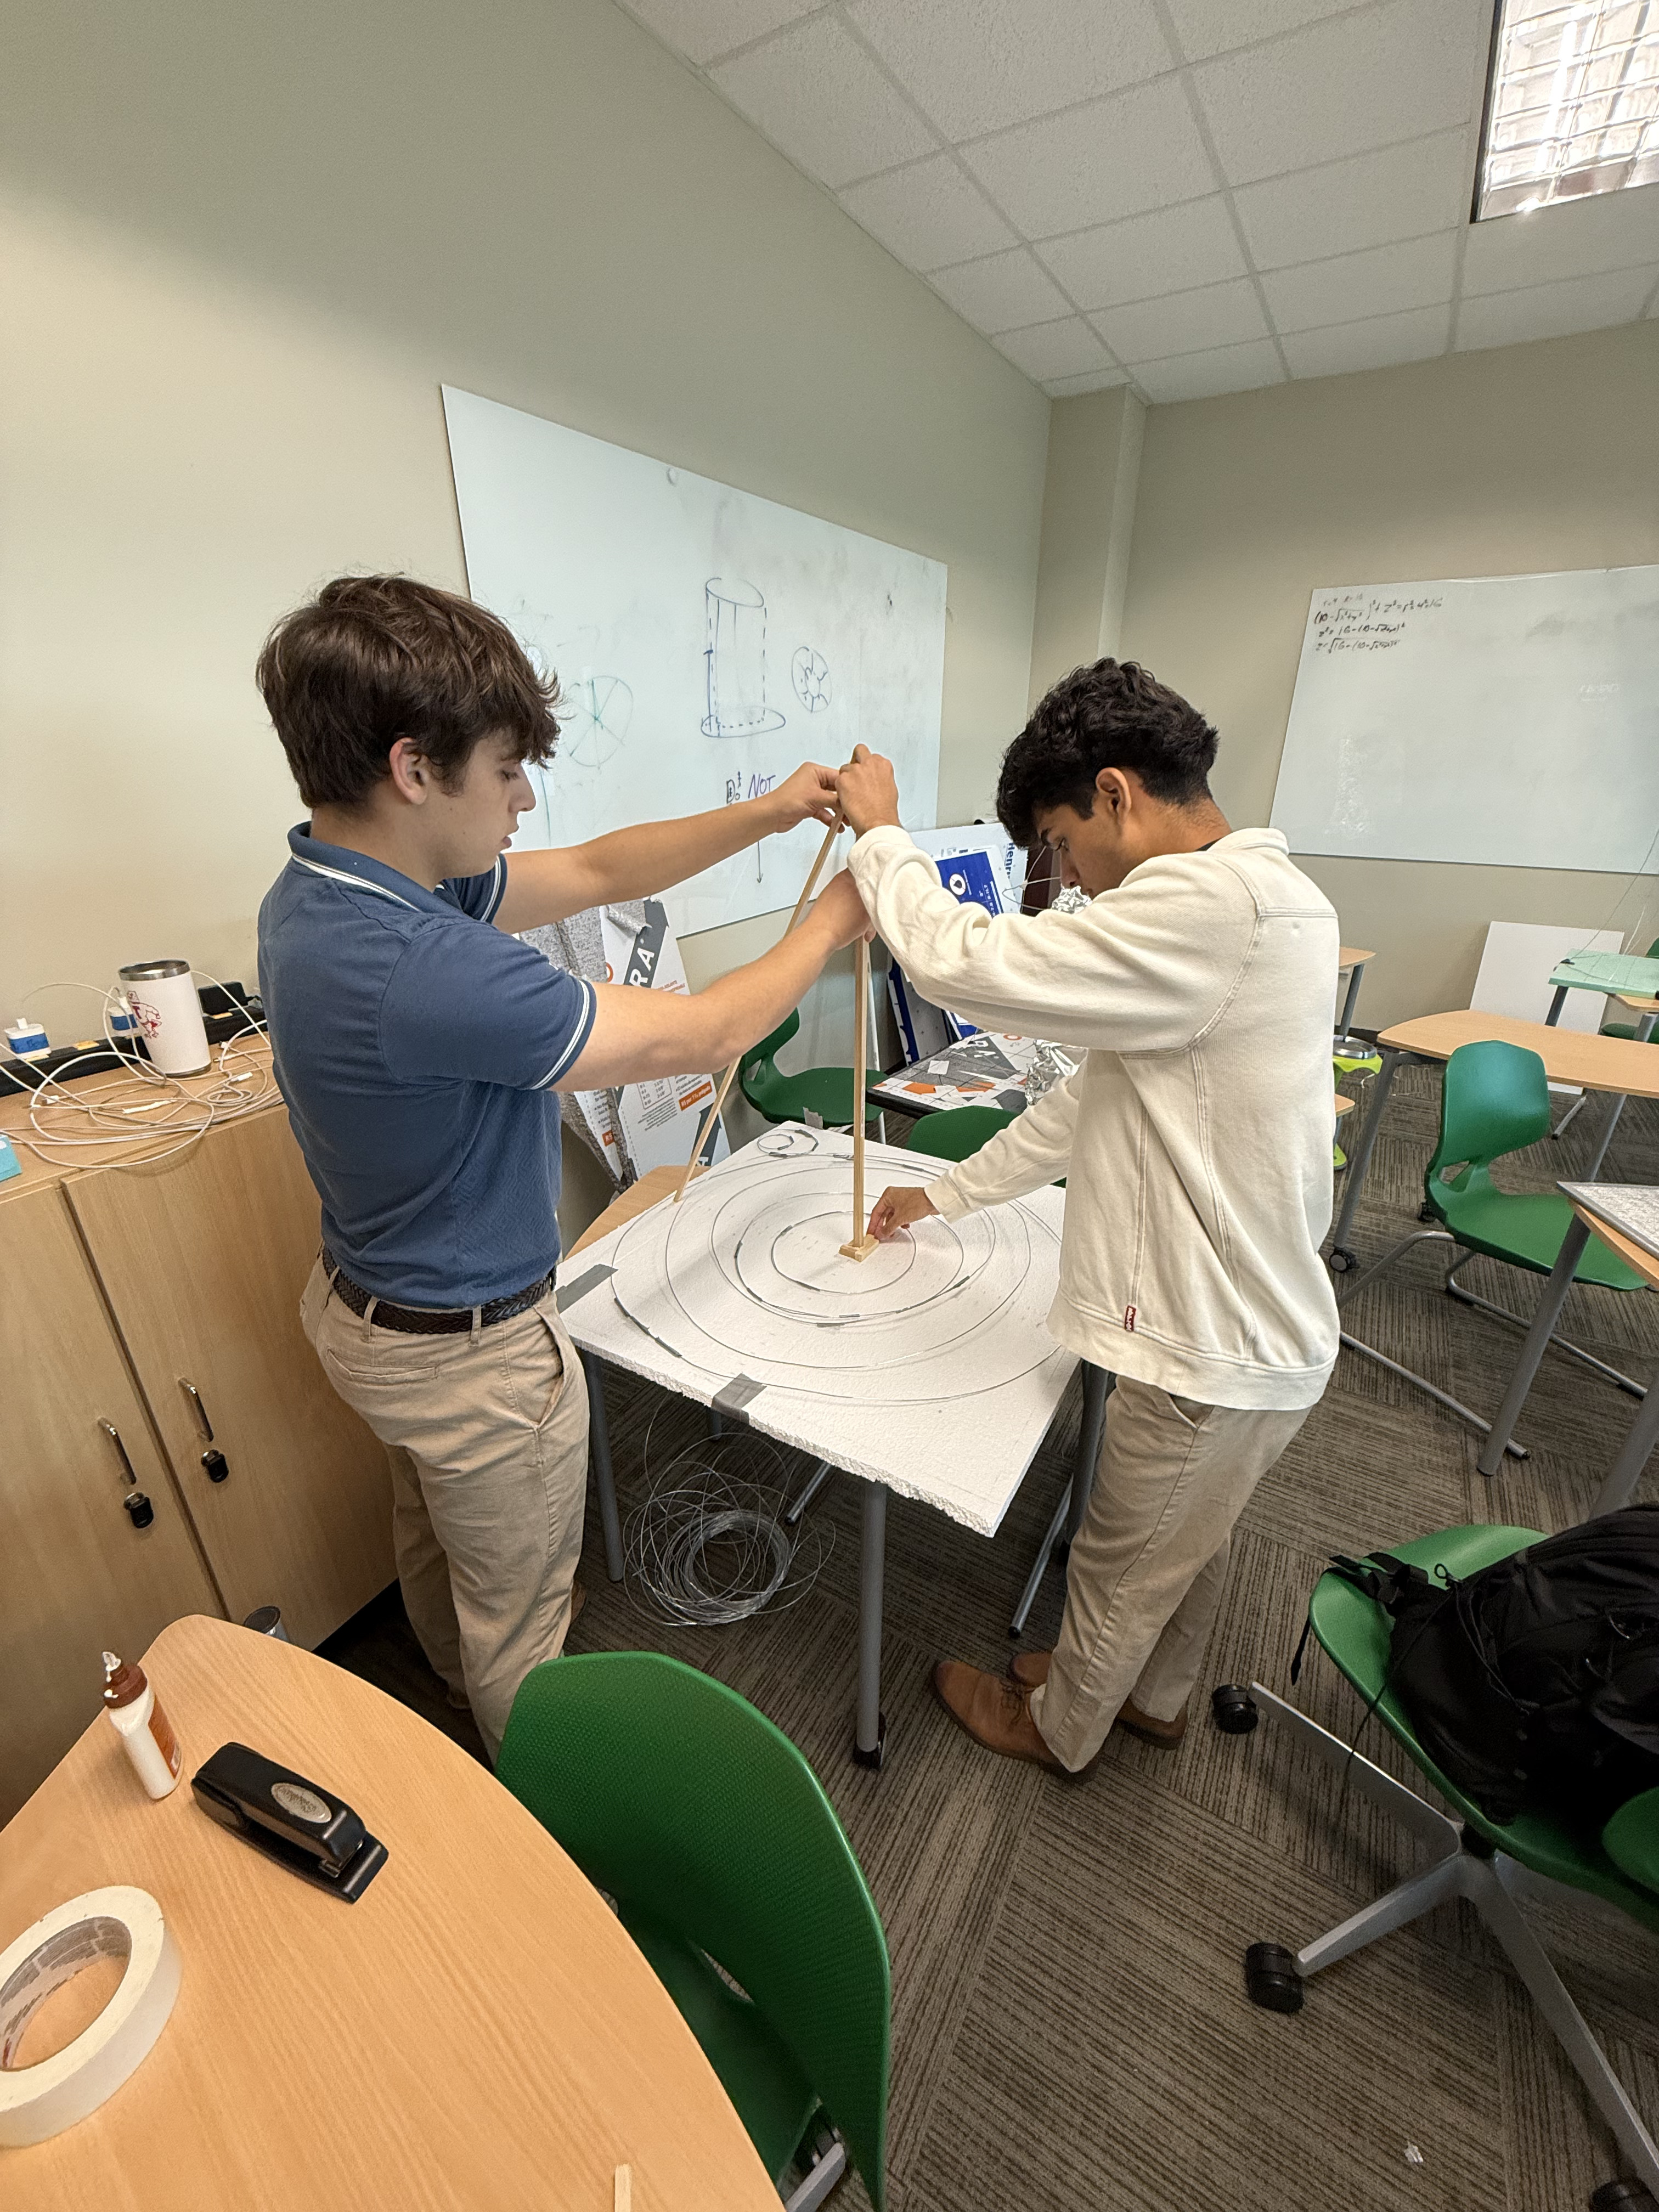
\includegraphics[trim=0 500pt 0 500pt, clip, width=0.5\textwidth]{cone-construction}
    \caption*{Diego and Keshav working on the wooden sticks.}
    \label{fig:cone-construction}
\end{figure}

Afterwards, we started on our theme: ice cream. As the cone was constructed with
the peak radius at the base, instead of at the highest $z$ value, we decided to
go with a fallen ice cream cone. So we used white construction paper and brown
construction paper to wrap one half of the cone, and ripped pieces of green,
pink, yellow, blue, and red construction paper for the sprinkles. Our (almost)
finished product looked as follows:

\begin{figure}[h!]
    \centering
    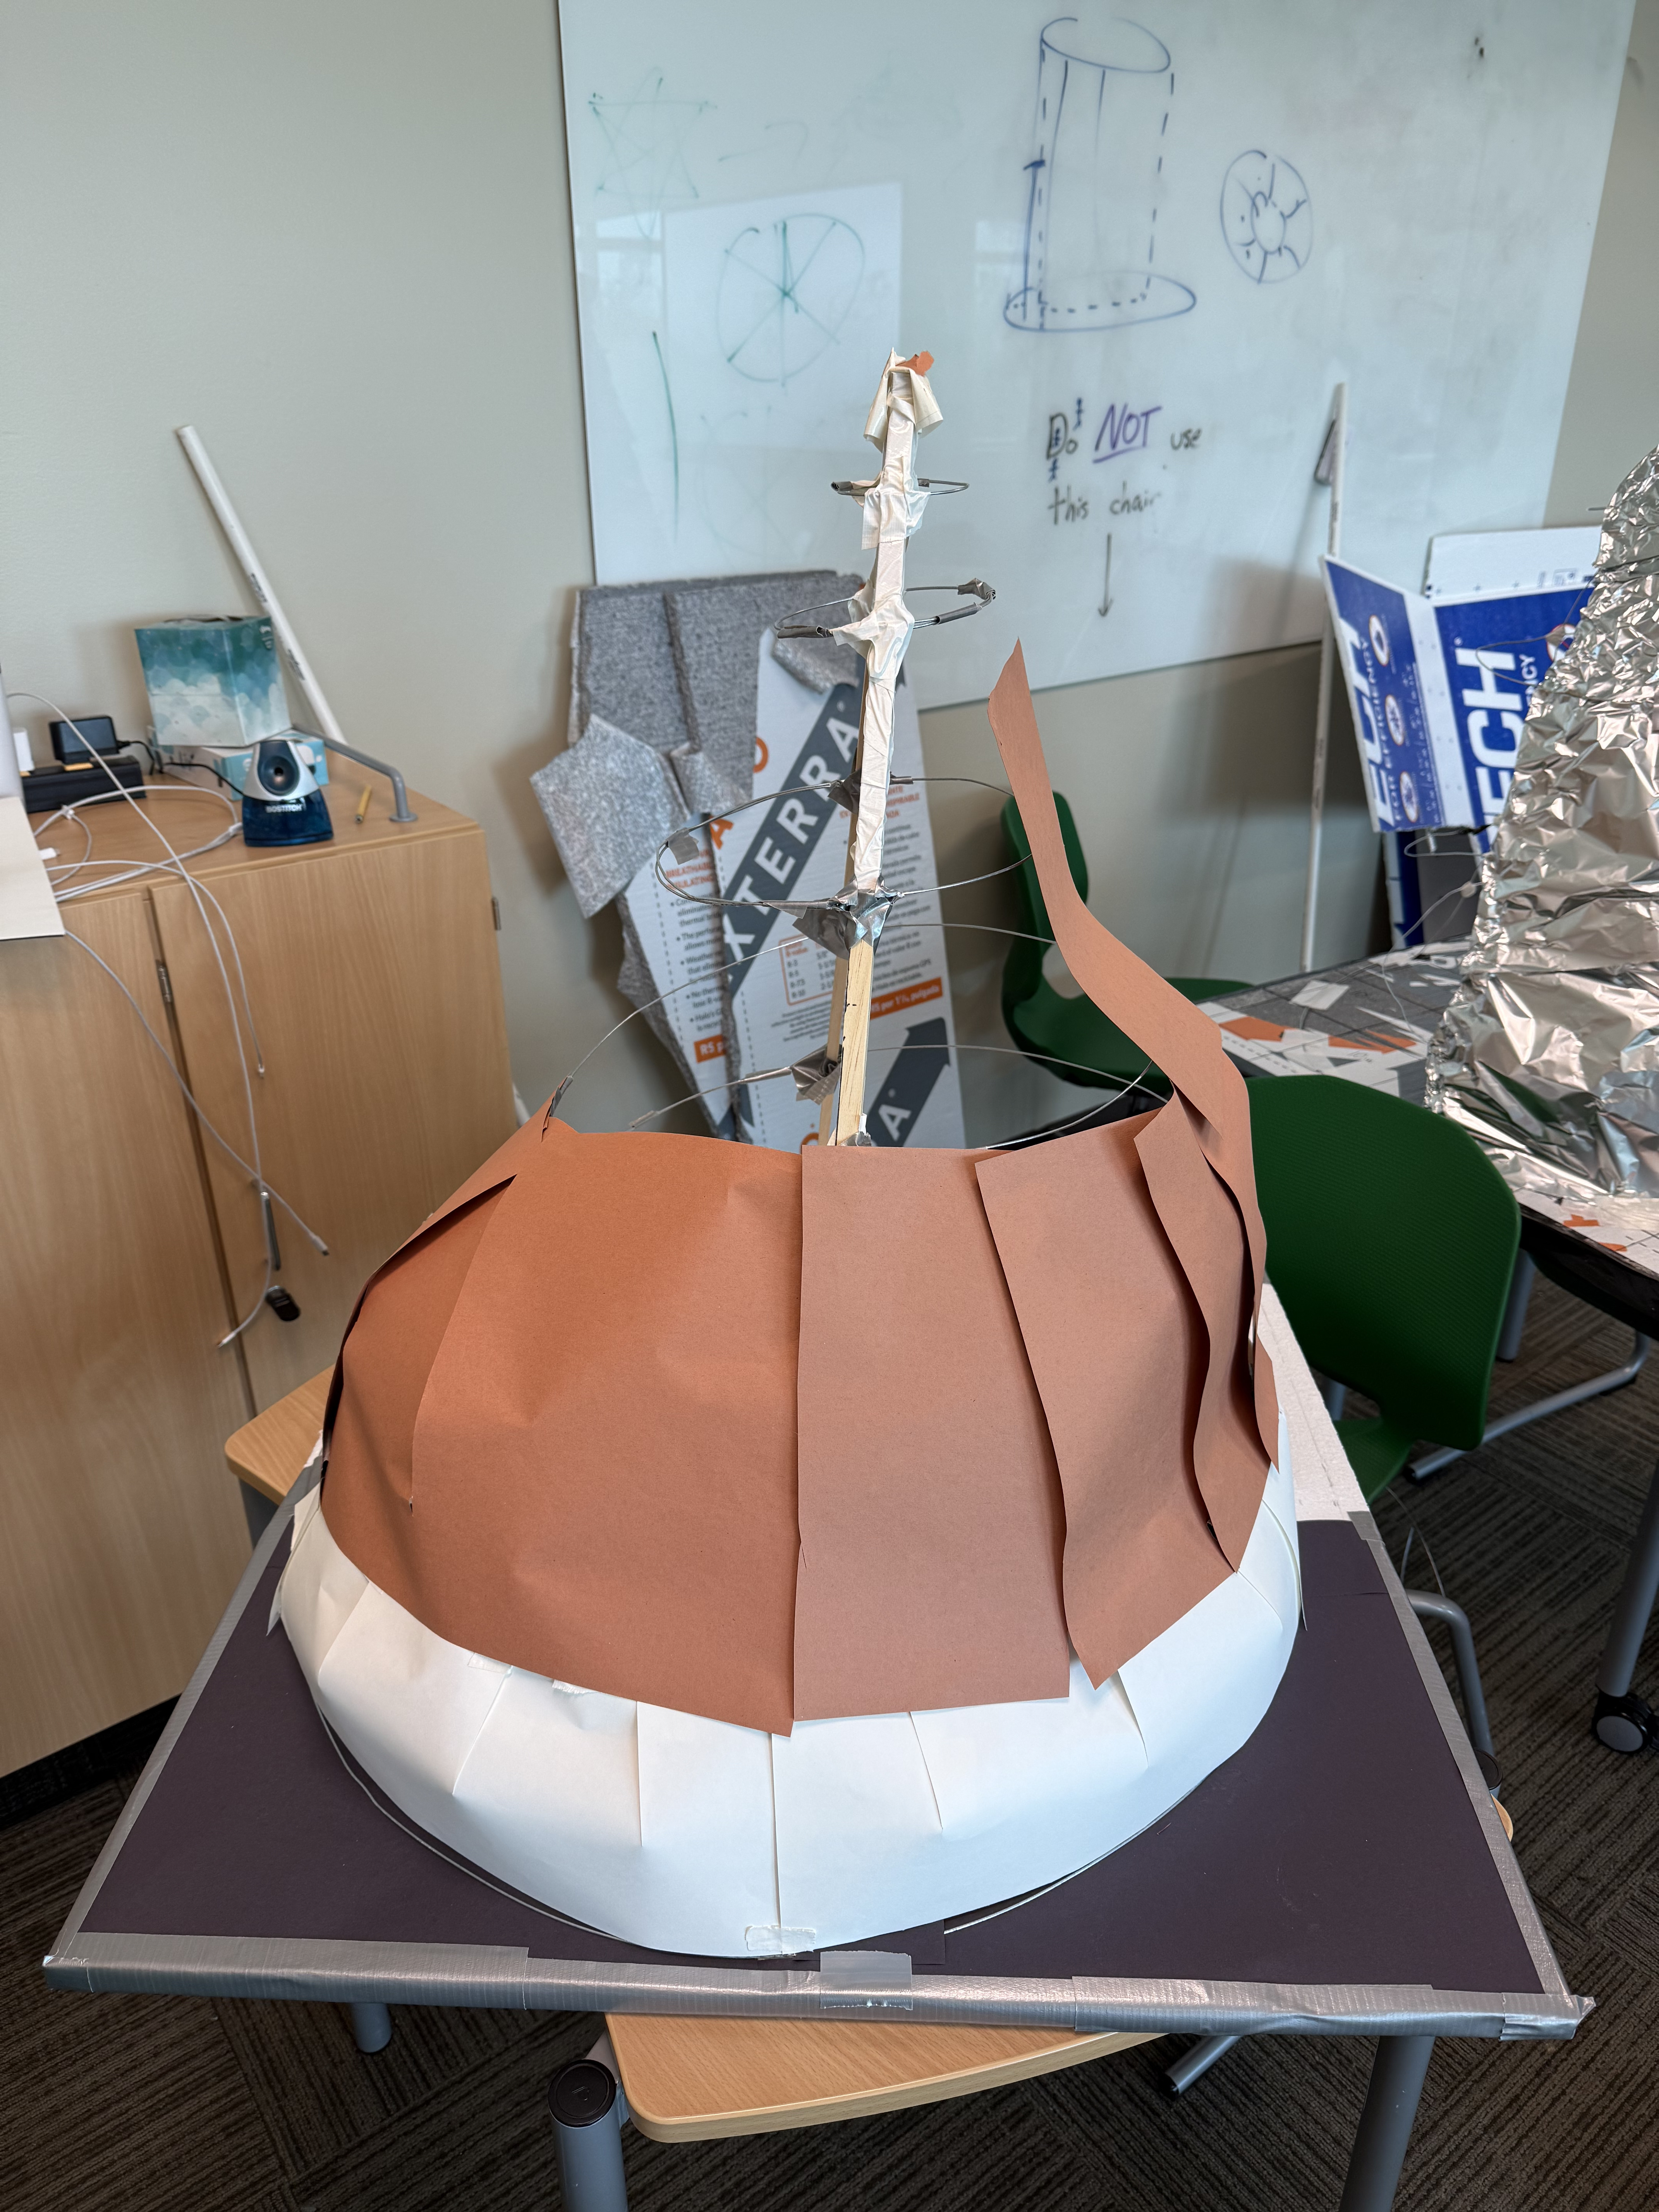
\includegraphics[trim=0 300pt 0 600pt, clip, width=0.5\textwidth]{cone-decoration}
    \caption*{The almost finished cone, without sprinkles.}
    \label{fig:cone-decoration}
\end{figure}

\clearpage

\section{Calculations}

\subsection{Theoretical Precise Volume}

To calculate the theoretical precise value, we will use the triple integral
\begin{equation*}
    \iiint\limits_{Q} f(x, y, z) \, dV.
\end{equation*}
To find the bounds, we will use cylindrical coordinates, as Cartesian
coordinates tend to end up messy in such calculations. To find the bounds in
cylindrical coordinates, we only need to solve for $r$, as $\theta \in [0,
2\pi]$ and $z \in [0, 30]$, as given by our domain restrictions above.

To find the bounds for $r$, we first convert the rectangular $x$ and $y$ to
cylindrical coordiantes. Following the conversion, our cone can be represented
by the equation $\frac{r^{2}}{225} = \frac{z^{2}}{900}$, which we can solve to
find the upper bound for $r$:
\begin{align*}
    \frac{r^{2}}{225} = \frac{z^{2}}{900} \implies r^{2} = \frac{225z^{2}}{900} \implies r = 
    \sqrt{ \frac{225z^{2}}{900} } = \sqrt{ \frac{z^{2}}{4} } = \frac{z}{2}.
\end{align*}

Thus, the upper bound for $r$ is $\frac{z}{4}$, and because the lower  
bound for $r$ is $0$, we know that the complete bounds for $r$ are $[0,
\frac{z}{4}]$. Thus, the complete bounds, for all variables, are:
\begin{equation*}
    \theta \in \left[ 0, 2\pi \right], \ z \in \left[ 0, 30 \right],  \ \text{and} 
    \ r \in \left[ 0, \frac{z}{2} \right].
\end{equation*}

Therefore, we can plug in the bounds and integrand for the triple integral and
evaluate it:
\begin{gather*}
    V = \int_{0}^{2\pi} \int_{0}^{30} \int_{0}^{\frac{z}{2}} r \, dr  \, dz  \, d\theta
    = \int_{0}^{2\pi} \int_{0}^{30} \left[ \frac{r^{2}}{2} \right]_{0}^{\frac{z}{2}} \, dz  \, d\theta
    = \int_{0}^{2\pi} \int_{0}^{30} \frac{z^{2}}{8} \, dz  \, d\theta \\
    = \int_{0}^{2\pi} \left[ \frac{z^{3}}{24} \right]_{0}^{30} \, d\theta
    = 1125 \int_{0}^{2\pi} \, d\theta
    = 1125 \, (2\pi)
    = 2250\pi
    \approx 7068.5835.
\end{gather*}

Thus, the theoretical precise volume of our cone is approximately $\boxed{
7068.5835 \ \text{cubic inches}}$ (or approximately $4.0906$ cubic feet).

\subsection{Theoretical Approximate Volume}

To calculate the theoretical approximate value of the equation
$\frac{x^{2}}{225} + \frac{y^{2}}{225} = (\frac{z^{2}}{900})$, we must first
convert to cylindrical coordinates to find the radius with respect to $z$, the
height. The radius $r$ can be found via the equations:
\begin{equation*}
    \frac{r^{2}}{225} = \frac{z^{2}}{900} \implies r^{2} = \frac{z^{2}}{4} \implies r = \frac{z}{2}.
\end{equation*}

To visualize the Riemann sum, imagine a layer cake with multiple layers that are
cylinders of arbitrary $h$ height, and gradually increasing radii. A  summation
of all the heights of every layer equates to $z$, or $30$. And, note that there
are $n$ cylinders. Additionally, at the peak of the inverted cone, or height
$30$, the radius is $15$, and at the minimum, or height $1$ (not including
height $0$), the radius is $\frac{1}{2}$. Now, for the formal calculation.

Let $r$ be the radius of the partition which is a cylinder, $h$ be the height,
$z$ be the height of the original cone, and $n$ be the number of partitions that
are taken, specifically referring to the height. The radius, with respect to
$z$, is $r = \frac{z}{2}$. The area of each cylinder's circle is
$\frac{z^{2}}{4}\pi$. Therefore, the area of each partition is
$\frac{z^{2}}{4}h\pi$. Finally, let $\Delta z_{0} = \frac{30 - 0}{n}$, and let
$z_{i} = i \Delta z_{0}$. Inputting all the values into the Riemann sum and
taking the limit of it is as follows:
\begin{gather*}
    V = \sum_{i=1}^{5} [f(z_{i})]^{2} \pi \Delta z_{0} 
    = \sum_{i=1}^{5} \frac{z_{i}^{2}}{4}\pi \Delta z_{0} 
    = \sum_{i=1}^{5} \frac{(i \Delta z_{0})^{2}\pi}{4} \Delta z_{0} 
    = \sum_{i=1}^{5} \frac{\pi}{4} i^{2} \Delta z_{0}^{3} 
    = \sum_{i=1}^{5} \frac{\pi}{4} i^{2} \frac{30^{3}}{5^{3}} \\
    = \sum_{i=1}^{5} \frac{\pi}{4} i^{2} \frac{27000}{5^{3}}
    = \sum_{i=1}^{5} \frac{6750\pi}{5^{3}} i^{2}
    = \frac{6750\pi}{125}(1^{2}) + \frac{6750\pi}{125}(2^{2}) + \dots + \frac{6750\pi}{125}(5^{2})
    \approx 9330.5302
\end{gather*}

The theoretical approximate volume of our cone is approximately
$\boxed{9330.5302 \ \text{cubic inches}}$ (or approximately $5.3996$ cubic
feet).

\subsection{Actual Approximate Volume}

To calculate the actual approximate volume, we'll use the same method that we
used for the theoretical approximate volume, as both are approximate. We'll
calculate the volumes of each partition (a cylinder) and add them up. The radii
that we recorded, in order from the base to the point, were $12"$, $9"$, $7"$,
$5"$, $2.5"$, and $1"$, and the heights of each circle that we recorded were
$5"$, $4"$, $6"$, $6"$, $5.5"$, and $3"$, respectively. Thus, the calculations
can be found via the summation
\begin{gather*}
    V = \sum \pi r^{2} (h) = 12^{2} \pi (5) + 9^{2} \pi (4) + \dots + 1^{2} \pi (3)
    \approx 4718.4896
\end{gather*}

Our actual approximate volume is roughly $\boxed{4718.4896 \ \text{cubic
inches}}$ (or $2.7306$ cubic feet).

\clearpage

\section{Discussion}

\subsection{Theoretical Precise Volume}

Our theoretical precise volume is $7068.5835$ cubic inches, and the volume makes
sense for the shape that we're planning to construct. Because the volume of the
cylinder with $r = 15"$ and $z = 30"$ can be found via the calculations
\begin{equation*}
    V = \pi r^{2} z = \pi 15^{2} (30) = \pi 225 (30) = 6750 \pi,
\end{equation*}
and the final volume is approximately $21205.7504$ cubic inches. The volume of
our cone is thus contained in the volume of the cylinder, which is logical and
appropriate.

\subsection{Theoretical Approximate Volume}

Our theoretical approximate volume, found with the Riemann sum $\sum_{i=1}^{5}
\frac{6750\pi}{125} i^{2}$ yielded the volume $9330.5302$ cubic inches, which
makes sense, as we took the cylinders of $h$ height stacked on top of each
other, from the base of the cone to the point. Those cylinders are an
overestimate, as they were calculated by finding the radius at the base of each
cylinder and extending the area of the base to height $h$, effectively leaving
the base area at the next point as well.

To find the percent error of our theoretical approximate volume, we can use the
formula for percent error:
\begin{gather*}
    \text{Percent Error}
    = \left| \frac{\text{Measured Value} - \text{True Value}}{\text{True Value}} \right| \times 100\%.
\end{gather*}
Our true value would be the value of the integral, $7068.5835$, and our measured
value would be the value of the Riemann sum, our theoretical approximate value,
$9330.5302$. The resulting calculations, with those numbers plugged in, would
be:
\begin{gather*}
    \text{Percent Error} 
    = \left| \frac{9330.5302 - 7068.5835}{7068.5835} \right| \times 100
    = \left| \frac{2261.9467}{7068.5835} \right| \times 100 \\
    = \left| 0.3199999972 \right| \times 100
    \approx 32 \%
\end{gather*}

Thus, our theoretical approximate volume's percent error is approximately
$\boxed{32\%}$.

\subsection{Actual Approximate Volume}

Because we calculated our actual approximate volume with a Riemann sum that took
partitions with radii based on the highest point of the partition, whereas when
we calculated our theoretical approximate value, we took Riemann sum partitions
with radii based on the lowest point of partition. The difference led to the
sums being under- and overestimates, respectively. View the actual approximate
volume as the right Riemann sum on decreasing function, leading to an
underestimate, but view the theoretical approximate volume as a left Riemann sum
on the same decreasing function.

Therefore, it makes sense that our actual volume was less than the triple
integral, but the theoretical approximate volume was greater than the triple
integral. So, we can calculate our percent error and assume that the percent
error will be roughly around the percent error for the theoretical approximate
value. The calculations are as follows:
\begin{gather*}
    \text{Percent Error} 
    = \left| \frac{4718.4896 - 7068.5835}{7068.5835} \right| \times 100
    = \left| \frac{2350.0939}{7068.5835} \right| \times 100 \\
    = \left| 0.332470275 \right| \times 100
    \approx 33 \%
\end{gather*}

So, we can see that the percent errors are approximately the same, just in
conceptually different directions, one an underestimate, and the other an
overestimate. Thus, our actual approximate volume's percent error is
$\boxed{33\%}$.

\end{document}
